% !TEX root = ../main.tex

\section*{1}
We give the algorithm as follows. \\

\begin{itemize}
    \item Given a simple polygon $P$ a with $n$ vertices.
    \item Perform triangulation on $P$.
    \item Construct the dual graph $G$ of $P$.
    \item Find a root node $R$ of $G$ whose degree is 1.
    \item Perform $LabelNumberOfChildNodes(G,R)$, which is described in 
      \ref{alg:LabelNumberOfChildNodes}.
    \item Select the node $v_i$ whose label is $n$ where $n = max(label_i,0<i<n \text{ and } label_i \leq \lfloor 2n/3\rfloor )$
    \item Find the diagonal line corresponding to the edge between $v_i$ and its parent.
\end{itemize}

\begin{algorithm}[h]
  \caption{LabelNumberOfChildNodes}
  \label{alg:LabelNumberOfChildNodes}
  \begin{algorithmic}
      \Require a dual graph $G$ and a node $v_i$
      \State Label $v_i$ as $Visited$
      \If{$degree(v_i) > 1 $}
      \State $NumNodes = 0$
      \For{Each neighbor $v_j$ of $v_i$}
      \If{$v_j$ is not $Visited$}
      \State $NumNodes$ = $NumNodes + LabelNumberOfChildNodes(G, v_j)$
      \EndIf
      \EndFor
      \State $label_i = 1 + NumNodes$
      \State Return $label_i$
      \Else
      \State $label_i = 1$
      \State Return $label_i$
      \EndIf
\end{algorithmic}
\end{algorithm}

\subsection*{Correctness}
The first case is when we can pick the node with the exact label, that is $\lfloor2n/3\rfloor$.
In this case, one polygon that the algorithm returns has exactly $\lfloor2n/3\rfloor + 2$ vertices. 
The other polygon has exactly $\lfloor n/3\rfloor + 2$ vertices.
Hence the algorithm is correct. \\

The second case, shown in Figure \ref{fig:extremecase}, is when we cannot find the exact label, so we have to find the closest node $v^*$, whose 
label is the maximum one that is less than $\lfloor2n/3\rfloor$. In this case, there is 2 branches starting
from the parent of $v^*$. Hence, the label of the parent of $v^*$ is the sum of the labels of its 2 children, 
and it is greater than $\lfloor2n/3\rfloor$. Therefore, if $v^*$ is the maximum value between the 2 children, 
then the label of $v^*$ is greater than $\lfloor n/3 \rfloor$. That is,

$$n/3 \leq label(v^*) < 2n/3$$

So if we cut by the edge between $v^*$ and its parent, neither of the 2 polygons has more than $\lfloor2n/3\rfloor + 2$ vertices.
Then the algorithm is correct. \\

\begin{center}
    \label{figure1}
    \begin{figure}[h]
    \centering
    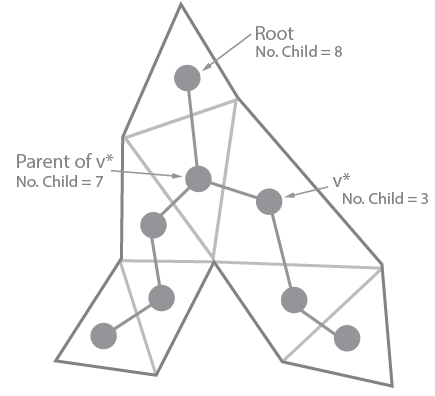
\includegraphics[width=5cm]{extreme-case}\\
    \caption{A polygon whose the tree of its dual graph has 2 branches} \label{fig:extremecase}
    \end{figure}
\end{center}

% Attach image

\subsection*{Running Time}
\begin{itemize}
    \item Performing triangulation on $P$ takes $O(n\log{n})$ (by splitting into y-monotone polygons and triangulate each one)
    \item Constructing the dual graph $G$ of $P$ takes $O(n)$
    \item Finding a root node $R$ of $G$ whose degree is 1 takes $O(n)$
    \item Performing $LabelNumberOfChildNodes(G,R)$ takes $O(n)$ because we traverse each node only once
    \item Selecting the appropriate node $v_i$ take $O(n)$
    \item Finding the diagonal line corresponding to the edge between $v_i$ and its parent takes constant time
\end{itemize}

Thus, the algorithm performs in $O(n\log{n})$
